% AGNTCY SLIM paper main LaTeX source (arXiv submission format)
\documentclass{article}
\usepackage{PRIMEarxiv}

% Encoding and typography
\usepackage[T1]{fontenc}
\usepackage[utf8]{inputenc}
\usepackage{microtype}
\usepackage{lmodern}
\usepackage{inconsolata} % mono font

% Math & symbols
\usepackage{amsmath, amssymb, amsthm}
\usepackage{mathtools}
\usepackage{bm}

% Graphics & figures
\usepackage{graphicx}
\usepackage{subcaption}
\usepackage{float}
\usepackage{tikz}
\usetikzlibrary{arrows.meta, positioning, calc, fit, shapes, backgrounds}

% Tables
\usepackage{booktabs}
\usepackage{multirow}
\usepackage{tabularx}
\usepackage{longtable}
\usepackage{threeparttable}
\usepackage{makecell}

% References & hyperlinks
\usepackage{hyperref}
\hypersetup{colorlinks=true, linkcolor=blue, citecolor=teal, urlcolor=magenta}
\usepackage[nameinlink,capitalize]{cleveref}

% Lists
\usepackage{enumitem}
\setlist{nosep}

% Code listings (placeholder; can swap for minted if shell access)
\usepackage{listings}
\lstset{basicstyle=\ttfamily\small,breaklines=true,frame=single}

% Acronyms / glossary
\usepackage[acronym]{glossaries}
\makeglossaries

% Bibliography (we'll generate a .bib later)
\usepackage[numbers,sort&compress]{natbib}

% Draft watermark (disable for submission)
%\usepackage{draftwatermark}
%\SetWatermarkText{DRAFT}
%\SetWatermarkScale{0.9}

% ---------- Metadata ----------
\title{AGNTCY SLIM: Secure Low-Latency Interactive Messaging for Distributed Agentic AI Systems}

\author{Luca Muscariello \\ Cisco \\ \texttt{lumuscar@cisco.com}
  \and Michele Papalini \\ Cisco \\ \texttt{micpapal@cisco.com}
  \and Mauro Sardara \\ Cisco \\ \texttt{msardara@cisco.com}}

\date{September 2025}

% Abstract macro (allows reuse if needed)
\newcommand{\SLIM}{\textsc{SLIM}}
\newcommand{\MLS}{\textsc{MLS}}
\newcommand{\HTTP}{HTTP/2\slash3}

% Glossary entries (initial set; expand later)
\newacronym{slim}{SLIM}{Secure Low-Latency Interactive Messaging}
\newacronym{mls}{MLS}{Messaging Layer Security}
\newacronym{did}{DID}{Decentralized Identifier}
\newacronym{grpc}{gRPC}{Google Remote Procedure Call}
\newacronym{qos}{QoS}{Quality of Service}

% Theorems (if needed for any formal statements)
\theoremstyle{definition}
\newtheorem{definition}{Definition}
\theoremstyle{remark}
\newtheorem{remark}{Remark}

\begin{document}
\maketitle
\begin{abstract}
We present \gls{slim}, a messaging protocol conceived for real-time, secure, many-to-many interaction among autonomous and human-assisted AI agents. Built atop gRPC over \HTTP{} and group cryptography via \gls{mls}, \gls{slim} integrates hierarchical routable naming, end-to-end protected streaming, and dynamic membership management. The protocol addresses gaps in existing messaging systems (enterprise queuing, IoT pub/sub, cloud-native buses, and log-centric streaming) by combining low-latency multiplexed transport with cryptographic group semantics offering forward secrecy, post-compromise security, and quantum-safe readiness. We articulate the architectural model (nodes, control plane, session layer), naming and routing scheme, reliability spectrum, and security properties, and position \gls{slim} relative to AMQP, MQTT, NATS, Kafka, and WebSocket-tunneled variants. We outline an evaluation methodology and a roadmap toward broader ecosystem interoperability and optional persistence extensions.
\end{abstract}


% 1. Introduction
\section{Introduction}\label{sec:intro}
Multi-agent AI systems increasingly perform time-sensitive coordination, tool invocation, collaborative reasoning, and continuous streaming of partial results (e.g., token generation, sensor fusion). Current messaging infrastructures each address subsets of these requirements but fall short when combining: (i) low tail latency under concurrency, (ii) cryptographic group guarantees across trust boundaries \citep{rfc9420,rfc9750}, (iii) hierarchical multi-tenant naming with aggregatable routing \citep{rfc6920,didcore}, and (iv) seamless bidirectional streaming plus request/response within a unified abstraction leveraging widely deployed transports (gRPC \citep{grpc}, HTTP/2 \citep{http2}). \gls{slim} is designed as a convergence layer to reconcile these dimensions while reusing existing operational ecosystems.

\subsection{Contributions}
This paper contributes: (1) a cohesive architectural decomposition of \gls{slim}; (2) a formalized hierarchical naming and channel moderation model leveraging \gls{did}-based identifiers \citep{didcore,didmethods,didkey}; (3) an analysis of the reliability and streaming semantics over a multiplexed secure transport; (4) security and threat modeling grounded in \gls{mls} properties (forward secrecy, post-compromise recovery) \citep{rfc9420,rfc9750}; (5) comparative positioning vs established protocols (AMQP \citep{amqp10}, MQTT \citep{mqtt311}, NATS \citep{nats}, Kafka \citep{kafka}, ActivityPub \citep{activitypub}, Matrix \citep{matrixspec}, XMPP \citep{xmpp-core}, Nostr \citep{nostr}); (6) an evaluation blueprint for future empirical study.

% 2. Motivation and Problem Statement
\section{Motivation and Problem Statement}\label{sec:motivation}
We summarize workload drivers: token-level streaming, dynamic membership churn, cross-organizational enclaves, partial-state sharing, and need for cryptographic agility. Threat considerations include untrusted intermediaries, malicious or compromised agents, replay attempts, namespace squatting, and future quantum adversaries. Existing systems typically rely on transport-only TLS, lack granular hierarchical naming semantics tied to identity, and impose operational overhead or complexity mismatched to agile agent ecosystems.

% 3. Design Goals
\section{Design Goals}\label{sec:goals}
We enumerate core goals: low-latency multiplexing; strong end-to-end and group confidentiality/integrity (MLS \citep{rfc9420}); efficient membership operations; globally unique aggregatable naming (hash/content-derived identifiers \citep{rfc6920}); reuse of HTTP/gRPC operational tooling (\citep{grpc,http2}); reliability spectrum (fire-and-forget through exactly-once); decentralized and federated identity support (DID ecosystem \citep{didcore,didmethods}); optional broker plus peer-to-peer adaptability; observability alignment. Normative requirement keywords follow \citep{rfc2119,rfc8174}.

% 4. Architecture Overview
\section{Architecture Overview}\label{sec:architecture}
\subsection{Component Roles}
\paragraph{Messaging Nodes.} A \emph{messaging node} is an application-layer router specialized for secure group traffic. Each node maintains (i) a \emph{connection table} (live client and peer node sessions with cryptographic / capability metadata) and (ii) a \emph{subscription table} (compressed mapping from hierarchical channel prefixes to next hops and locally attached subscribers). Unlike traditional brokers that couple durability with routing, a SLIM node focuses on low-latency forwarding of already end-to-end protected content; persistence (if desired) can be introduced as an orthogonal extension (\S\ref{sec:future}).
\paragraph{Producers / Consumers.} Agents frequently act in a dual capacity: publishing intermediate reasoning artifacts while simultaneously consuming observations, tool outputs, or peer proposals. SLIM therefore avoids hard role separation---the session layer exposes a symmetric API where `publish`, `subscribe`, and streaming primitives coexist.
\paragraph{Control Plane.} The control plane provides node discovery, distribution of connection/subscription deltas, organizational policy enforcement, telemetry collection, and global health signaling. A logically centralized service may implement this for early deployments; federation (multi-organization peering) composes via signed policy bundles.
\paragraph{Session Layer Library.} Client libraries encapsulate MLS state machines, channel membership persistence, reconnect logic, reliability modes, and backpressure adaptation (window sizing, application-level flow hints).
\paragraph{Cryptographic Services.} MLS authentication / delivery services are \emph{logical} functions: issuance / validation of credentials and relay of MLS commit messages. In some deployments these functions collocate with the control plane; in others they are decentralized.

\subsection{Plane Separation (Data vs Control)}
Data-plane paths transport encrypted application payloads; control-plane channels transport low-rate topology, membership, and policy updates. Decoupling yields: (a) different scaling elasticity (add nodes to meet throughput while leaving governance capacity intact), (b) failure domain isolation (control-plane glitch does not stall in-flight secure streams), and (c) observability clarity (distinct SLOs for message latency vs configuration convergence time).

\subsection{Core Tables and their Dynamics}
The connection table is a time-varying graph adjacency representation: entries contain peer identity (DID or derived hash), negotiated protocol version, QoS preferences, liveness timers, recent throughput counters, and MLS group participation references. The subscription table is a compressed Patricia / radix style structure keyed by hierarchical channel components; entries hold forwarding vectors (set of next-hop nodes) plus local subscriber sets. Aggregation is performed whenever multiple concrete channel names share a longest common organizational prefix without conflicting policy constraints.

\subsection{Name-Centric Routing Rationale}
SLIM adopts hierarchical names rather than opaque UUID topics to enable (1) routing table compression, (2) policy scoping using prefix semantics (e.g., deny `did:key:ORG/finance/*`), and (3) discoverability under controlled exposure (agents can list permissible namespace branches). Cryptographic binding between names and key material mitigates impersonation and prefix squatting.

\subsection{Illustrative Topology}
\begin{figure}[H]
  \centering
  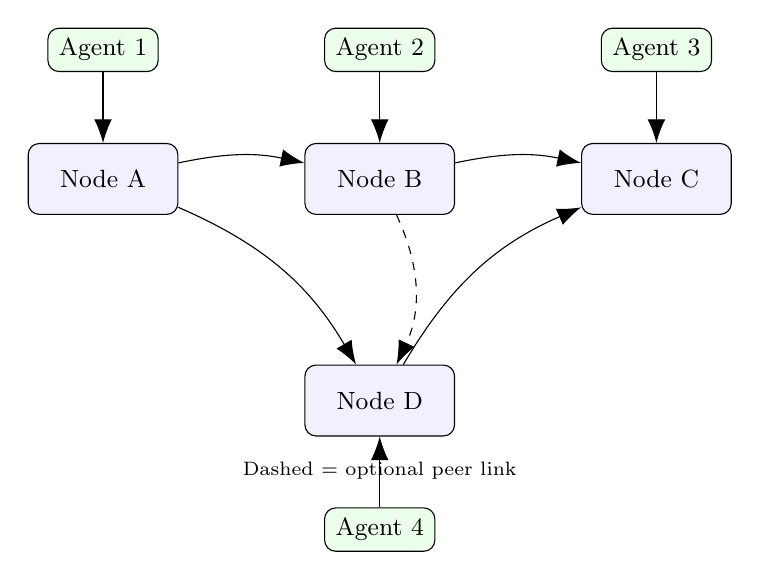
\begin{tikzpicture}[node distance=1.9cm and 1.6cm, every node/.style={font=\small}]
    	\tikzstyle{n}=[draw,rounded corners,minimum width=1.9cm,minimum height=0.9cm,fill=blue!6]
    	\tikzstyle{a}=[draw,rounded corners,minimum width=1.4cm,minimum height=0.55cm,fill=green!8]
    \node[n] (n1) {Node A};
    \node[n,right=of n1] (n2) {Node B};
    \node[n,right=of n2] (n3) {Node C};
    \node[n,below=of n2] (n5) {Node D};
    \node[a,above=0.9cm of n1] (p1) {Agent 1};
    \node[a,above=0.9cm of n2] (p2) {Agent 2};
    \node[a,above=0.9cm of n3] (p3) {Agent 3};
    \node[a,below=0.9cm of n5] (p4) {Agent 4};
    \draw[-{Latex[length=3mm]}] (p1) -- (n1);
    \draw[-{Latex[length=3mm]}] (p2) -- (n2);
    \draw[-{Latex[length=3mm]}] (p3) -- (n3);
    \draw[-{Latex[length=3mm]}] (p4) -- (n5);
    \draw[-{Latex[length=3mm]},bend left=12] (n1) to (n2);
    \draw[-{Latex[length=3mm]},bend left=12] (n2) to (n3);
    \draw[-{Latex[length=3mm]},bend left=18] (n1) to (n5);
    \draw[-{Latex[length=3mm]},bend left=18] (n5) to (n3);
    \draw[-{Latex[length=3mm]},bend left=25,dashed] (n2) to (n5);
    \node[below=0.2cm of n5,align=center,font=\scriptsize] {Dashed = optional peer link};
  \end{tikzpicture}
  \caption{Example multi-node deployment with agents attached at edge nodes and aggregated route advertisement of organizational prefixes.}
  \label{fig:topology}
\end{figure}

% 5. Naming and Routing Model
\section{Naming and Routing Model}\label{sec:naming}
\subsection{Identifier Classes}
Three principal identifier sets exist: (1) \emph{node identifiers} (onboarding / mutual authentication), (2) \emph{client locators} (agent endpoints), and (3) \emph{channel names} (MLS group scope + routing handle). Nodes require uniqueness but not aggregation; channels require both uniqueness \emph{and} aggregatable structure (content-hash / DID binding \citep{rfc6920,didcore}).
\subsection{Channel Schema}
Canonical form (illustrative) \citep{didcore,didkey}:
\begin{center}\ttfamily did:key:ORG/namespace/service/did:key:moderatorHash\end{center}
The trailing moderator DID binds the channel to a controlling principal authorized to stage membership changes. Prefixes up to `service` define aggregation boundaries for subscription compression.
\subsection{Client Locator Schema}
Similar structure substitutes the moderator DID with the client DID, allowing discovery queries scoped to organization or namespace. Hash-based references inhibit enumeration of unrelated branches while still enabling legitimate prefix discovery where policy permits.
\subsection{Aggregation and FIB Entries}
Nodes populate forwarding information base (FIB) entries for each active name prefix in which they have either (a) a downstream subscriber or (b) a peer advertising further sub-prefix reachability. Aggregation merges adjacent subtrees when next-hop sets are identical and policy tags align.
\subsection{Security Side Effects}
Name---key binding thwarts impersonation; DID resolution (e.g., via `did:web` or `did:key`) offers verifiability without relying on centralized PKI trust anchors \citep{didweb,didkey}. Collision resistance relies on the underlying cryptographic hash domain of the DID method; compromise would require second preimage for a published moderator key.

% 6. Protocol Operations
\section{Protocol Operations}\label{sec:operations}
\subsection{Group Lifecycle}
  	extbf{Create:} Moderator generates initial MLS group, advertises channel name; control plane optionally records metadata (policy tags). \textbf{Join:} Candidate presents credential; moderator (or delegated policy agent) issues MLS add commit disseminated via nodes (per \citep{rfc9420,rfc9750}). \textbf{Leave / Eject:} Removal triggers MLS update commit; nodes immediately drop cached state associated with the expelled member identity. \textbf{Epoch Advancement:} Every membership or key schedule change increments group epoch, enabling out-of-order delivery detection.
\subsection{Publish Flow}
1) Application serializes payload (e.g., Protocol Buffers). 2) Session layer wraps with per-message metadata (channel ID, reliability mode, correlation ID). 3) MLS encrypts producing ciphertext + auth tag. 4) Node ingress performs prefix lookup -> forwarding set. 5) Egress nodes deliver to local subscribers or propagate further. No intermediate can decrypt.
\subsection{Subscribe / Resubscribe}
Subscriptions register interest in a concrete channel or prefix (policy permitting). The session layer persists subscription intents locally; upon reconnection it replays intents idempotently, receiving current epoch and optionally missed reliable messages (if retention configured at application level).
\subsection{Reliability Modes}
\begin{itemize}[leftmargin=*]
  \item \emph{FNF (Fire-and-Forget):} No acknowledgment; minimal latency path.
  \item \emph{Acked-Unreliable:} Lightweight receipt acknowledgment (used for adaptive rate control / backpressure but no retransmit guarantee).
  \item \emph{Exactly-Once:} Message identifiers (nonce + epoch + sender DID) plus deduplication cache at consumers; optional negative acknowledgment window for selective retransmission.
\end{itemize}
Applications choose mode per message class, enabling fine-grained latency vs assurance trade-offs.
\subsection{Streaming Semantics}
gRPC streaming maps to sequences of MLS-protected frames under a single transport stream. Flow control leverages HTTP/2 window updates while the session layer enforces application-level quotas derived from observed RTT and backlog. Bidirectional streams permit interleaving of tool invocation results and agent refinements.
\subsection{Request / Reply Pattern}
Implemented as a pair of messages sharing a correlation identifier; reliability can elevate request or reply independently (e.g., reliable request with opportunistic reply).
\subsection{Error Handling}
Structured error codes: authentication failure, authorization denied, epoch mismatch, replay suspicion, backpressure throttle, unsupported protocol feature. Transient classes trigger exponential backoff; permanent classes escalate to the application.

% 7. Session Layer
\section{Session Layer}\label{sec:session}
The session layer mediates between application logic and low-level secure transport operations.
\subsection{Functional Responsibilities}
\begin{enumerate}[leftmargin=*]
  \item \textbf{MLS State Management:} Maintains current epoch, provisional pending commits, and cryptographic material; handles silent discard of stale epochs.
  \item \textbf{Channel Subscription Registry:} Idempotent store of active subscriptions with replay on reconnect.
  \item \textbf{Reliability Orchestration:} Tracks unacknowledged reliable transmissions, schedules retries or failure callbacks.
  \item \textbf{Flow Control Integration:} Bridges HTTP/2 stream/window signals to application-level rate adjustments.
  \item \textbf{Crash / Disconnect Recovery:} Persists minimal durable state (membership snapshot, pending reliable messages) enabling fast resumption.
\end{enumerate}
\subsection{API Surface Principles}
Asynchronous futures/promises for publish acknowledgments; streaming iterators for token-by-token inference data; explicit cancellation to assist cooperative load shedding.
\subsection{Backpressure Strategy}
Combines (a) consumer acknowledgment pacing, (b) dynamic window scaling, and (c) drop policies for FNF streams under sustained congestion.

% 8. Security and Trust Model
\section{Security and Trust Model}\label{sec:security}
Security properties derive from layered mechanisms: OAuth-based authentication conveying MLS credentials, hierarchical naming semantics enforcing scope, and MLS group cryptography ensuring confidentiality and integrity.
\subsection{Identity and Authentication}
Agents obtain bearer tokens from an authorization service which embeds (or references) MLS credentials and proofs of possession (group semantics per \citep{rfc9420}). Nodes validate token signatures, check revocation lists, and extract allowed namespace prefixes. DID documents anchor public keys enabling decentralized validation without exclusive dependence on centralized certificate authorities (\citep{didcore,didmethods}).
\subsection{Authorization}
Policy rules combine prefix patterns with role attributes (e.g., moderator, observer, contributor). Evaluation occurs before subscription installation or message acceptance. Moderators possess extended capability to propose membership changes but not to bypass namespace policies.
\subsection{Confidentiality, Integrity, and Forward Secrecy}
MLS provides a ratcheting key schedule \citep{rfc9420}; each commit advances secrets so that compromise of a current state does not reveal prior plaintext (forward secrecy) and subsequent post-compromise epochs restore confidentiality (PCS) \citep{rfc9750}. All application data (including correlation identifiers) resides within the authenticated envelope, limiting traffic analysis to size/timing only.
\subsection{Revocation and Ejection}
Revoking a token halts future connection refresh; issuing an MLS removal commit invalidates the expelled member's ability to derive next epoch secrets. Immediate effect is bounded by propagation delay of the commit across nodes.
\subsection{Quantum-Safe Considerations}
Future MLS suites integrating post-quantum KEMs can be adopted with minimal application disruption since higher layers treat encryption opaque. Names remain stable while cryptographic material rotates.
\subsection{Threat Analysis}
\paragraph{Man-in-the-Middle:} Encrypted group messages plus signature validation on commits prevent undetected content manipulation. \paragraph{Replay:} Epoch and per-message nonce semantics enable detection of duplicate ciphertext. \paragraph{Forking:} Divergent subgroup creation attempts without valid moderator commits are rejected due to signature / membership proofs. \paragraph{Insider Exfiltration:} Least-privilege namespace policies limit reachable channels; ejection + PCS curtails blast radius. \paragraph{Downgrade:} Protocol version negotiation requires mutual support list intersection with integrity protection, preventing silent downgrade to weaker ciphers.

% 9. Performance and Scalability
\section{Performance and Scalability}\label{sec:performance}
\subsection{Latency Decomposition}
Total one-way latency: \( T = T_{net} + T_{ser} + T_{crypto} + T_{queue} + T_{sched} \). SLIM minimizes \(T_{ser}\) via compact binary encoding (gRPC framing \citep{grpc}) and reduces \(T_{queue}\) by eschewing disk persistence on the critical path. \(T_{crypto}\) is bounded by MLS AEAD + per-message nonce computation \citep{rfc9420}.
\subsection{Connection Multiplexing Efficiency}
Multiple logical streams share a single transport connection (HTTP/2 multiplexing \citep{http2}), eliminating repeated TLS handshakes and head-of-line blocking effects observed when separate connections are used for each agent pairing; prospective QUIC migration \citep{quic} offers further transport evolution.
\subsection{Subscription Aggregation Impact}
Empirical expectation (future evaluation): compression ratio improves with namespace depth; in synthetic hierarchies with branching factor \(b\) and depth \(d\), aggregated entries approach \(\mathcal{O}(b \cdot d)\) versus \(\mathcal{O}(b^d)\) naive enumeration.
\subsection{Membership Churn Cost}
MLS commit size scales roughly logarithmically with group size under tree-based ratchets; recomputation overhead amortized across members. Session layer pipelines application traffic with key schedule operations to hide latency.
\subsection{Scaling Strategies}
Horizontal node scaling combined with consistent hashing (or topology-aware partitioning) distributes subscription storage. Control plane diff dissemination enables incremental updates rather than full table rewrites.
\subsection{Backpressure and Rate Adaptation}
Acked-unreliable mode supplies feedback signals without incurring full reliable overhead; congestion heuristics adjust publish pacing and promote selective reliability only for critical message classes.

% 10. Interoperability and Ecosystem Positioning
\section{Interoperability and Ecosystem Positioning}\label{sec:comparison}
We position SLIM along axes: security depth (transport vs message), group dynamism, latency under concurrency, naming expressiveness, operational footprint, and streaming versatility.
\subsection{AMQP / AMQP over WebSockets}
Rich routing and durability but higher protocol verbosity and reliance on broker trust for message confidentiality (unless extended) \citep{amqp10}. Group membership cryptography is external; WebSockets variant adds framing overhead for browser reach.
\subsection{MQTT}
Ultra-lightweight and ideal for constrained edge scenarios \citep{mqtt311}; lacks native end-to-end group encryption and advanced membership semantics; topic wildcards support simple subscription patterns but limited hierarchical policy richness.
\subsection{NATS}
Low-latency core with flexible patterns (pub/sub, request/reply) \citep{nats}; message security remains transport-scoped; JetStream adds durability at complexity cost. Subject naming is flat relative to SLIM's structured DID-infused hierarchy.
\subsection{Kafka}
Excels at sustained high-throughput and replay \citep{kafka}; inherent log design introduces additional commit / fetch latency for ultra-interactive exchanges; group cryptography must be layered separately; topic partition model focuses on scalability over fine-grained membership agility.
\subsection{Emerging / Social Protocols}
ActivityPub \citep{activitypub}, Matrix \citep{matrixspec}, XMPP \citep{xmpp-core}, Nostr \citep{nostr} provide federation or social graph features; they typically prioritize message persistence or social semantics over low-tail-latency group cryptography optimized for high-frequency agent coordination.
\subsection{Summary}
SLIM's differentiator is the \emph{combination} of (a) hierarchical cryptographically bound naming (\citep{rfc6920,didcore}), (b) integrated MLS for dynamic secure groups (\citep{rfc9420,rfc9750}), and (c) transport reuse with efficient multiplexed streaming (\citep{grpc,http2})—rather than peak performance in a single axis (e.g., Kafka throughput \citep{kafka}) or minimal footprint (e.g., MQTT simplicity \citep{mqtt311}).

% 11. Reference Implementation and Tooling
\section{Reference Implementation and Tooling}\label{sec:implementation}
Outline client SDK abstraction layers, control plane service endpoints, integration hooks with agent orchestration frameworks (LangChain, LangGraph, AutoGen), simulation harness for multi-agent load generation.

% 12. Use Cases
\section{Use Cases}\label{sec:usecases}
Enumerate scenarios: collaborative planning, secure multi-organization enclave, edge sensor fusion, human-in-the-loop oversight, token-by-token model steering.

% 13. Evaluation Methodology
\section{Evaluation Methodology}\label{sec:evaluation}
Experimental design for future benchmarking: metrics (p50/p95 latency, join latency, rekey cost, throughput under churn), testbed (synthetic agent swarm), instrumentation (tracing, cryptographic timers), and comparison baselines.

% 14. Future Work
\section{Future Work}\label{sec:future}
Optional persistence extension, causal metadata embedding, adaptive QoS negotiation, QUIC adoption study, post-quantum rollout, formal verification of session layer invariants.

% 15. Related Work
\section{Related Work}\label{sec:related}
Survey group messaging cryptography, distributed pub/sub fabrics, named data paradigms (linking hash-based naming lineage), log-structured streaming systems.

% 16. Conclusion
\section{Conclusion}\label{sec:conclusion}
Reinforce \gls{slim}'s positioning as an integrative secure low-latency substrate, summarize distinctiveness, outline adoption path and standardization trajectory.

% 17. Glossary
\printglossaries

% 18. References
\bibliographystyle{unsrtnat}
\bibliography{references}

\end{document}
